\documentclass{article}
\usepackage{float}
\usepackage{graphicx}
\usepackage{caption}
\usepackage{placeins}
\usepackage{textcomp}

\title{Quality Threshold Clustering}
\date{Caso di studio anno 2018-2019}
\author{Ivan Diliso \\Matricola: 676366}

\graphicspath{ {./Images/} }
\captionsetup{justification=raggedright,singlelinecheck=false}


\begin{document}
    
    \maketitle
    \tableofcontents
    \newpage
    \section{Introduzione}
    Il software \textbf{Qt-Clustering} realizzato in Java permette di applicare 
    l'algoritmo di cluster Quality Threshold ad un insieme di dati estratti da 
    un database MySQL. 

    \paragraph{Quality Threshold} 
    Algoritmo alternativo per partizionare i dati. Richiede più potenza di
    calcolo rispetto a K-Means ma non richiede di specificare il numero di
    cluster a priori, e restituisce sempre lo stesso risultato quando si ripete
    diverse volte.
 
    \section{Applicazione principale}
    L'applicazine è divisa in due componenti principali
        \subsection{Server}
        Il server si occupa di eseguire le richieste di uno o più client
        fornendo ad essi le seguenti funzionalità:
            \begin{itemize}
                \item Caricare una tabella dal database specificandone il nome
                \item Eseguire il clustering dei dati caricati
                \item Visualizzare i dati e il risultato del clustering
                \item Salvare il risultato del clustering su file
                \item Caricare i dati del clustering da file
            \end{itemize}
        
        
        \subsection{Client}
        Il client si occupa di gestire una interaccia utente basata su linea di 
        comando che permette all'utente di:
            \begin{itemize}
                \item Connettersi al server specificando una porta (valore di 
                default 8080)
                \item Chiedere al server di eseguire una nuova operazione di
                clustering specificando nome della tabella, raggio e il nome del
                file dove salvare i risultati
                \item Caricare un clustering salvato su file specificando il
                nome del file
            \end{itemize}

        \paragraph{Nota} Le classi del package QtClient sono state modificate 
        in modo da utilizzare una nuova classe per la gestione dei menu e per 
        la gestione dell'input con vincoli e per permettere al client di fare 
        richieste al server tramite una unica operazione "serverCommand" 
        (Le specifiche sono presenti nel Javadoc)
        

    \newpage
    \section{Estensione}
    L'estenzione del progetto consiste su una Web Application basata sul
    framework Spring Boot, che permette di creare applicazioni web basate sul
    pattern architetturale MVC (Model View Controller). \\\\ L'applicazione è basata 
    sull'utilizzo di Servlet Java (tramite SpringBoot) 
    per servire le pagine web, non sarà più presente dunque un modello
     client server 
    basato su socket ma 
    il client sarà rappresentato da una pagina web che si interfaccerà con il
    server per l'esecuzione del clustering, il caricamento dei dati dal database 
    e il trasferimento dei dati.\\

    L'interfaccia della webapp è composta da pagine JSP che verranno mappate ai 
    metodi di una classe controllore, che gestirà le righieste GET e POST e
    la visualizzazzione di altre pagine JSP settando i relativi parametri.

        \paragraph{Servlet}
        Oggeto scritto in linguaggio Java che opera all'interno di
        un server web permettendo quindi la creazine di applicazioni web. L'uso 
        più frequente delle servlet è la generazione di pagine web dinamiche a 
        seconda dei parametri di richiesta inviati dal client browser 
        dell'utente al server
    
        \subsection{Web Server}
        E' stata utilizzata una versione che opera tramite il web server e 
        servlet container Tomcat embedded all'interno dell'applicazione. 
        In questo modo non ci sara' bisogno di avviare il web server Tomcat ma 
        bastera' avviare il WAR (Web Application Resource) del server per 
        avviare sia il web server, sia la web application

        \subsection{Libreria JSON}
        Per servire i dati del database e i risultati del clustering sono state
        create delle classi per la costruzione di file JSON. La libreria
        presenta una struttura ad albero per rappresentare i dati. Verrà poi 
        utilizzata la classe controllore per mappare i file JSON alle relative 
        pagine web

        \subsection{Interfaccia Web}
        L'interfaccia web è stata realizzata in HTML/CSS e presenta delle funzoni 
        in Javascript per trasformare i dati JSON forniti dal server in tabelle
        HTML.  È  stata utilizzata la libreria BOOTSTRAP per omoloagare la 
        grafica delle pagine web e fornire dei siti web responsive. \\\\
        È stata aggiunta la classe TableNames 
        per permettere di caricare dal database il nome di tutte le tabelle
        presenti e costruire una menu a tendina per la scelta della tabella da 
        utilizzare.






    \newpage
    \section{Installazione}
    Questi passaggi sono validi sia per il progetto base sia per il progetto con
    estensione.
    Sia il client sia il server necessitano l'installazione dei sequenti
    software:
        \begin{itemize}
            \item MySQL
            \item Java Runtime Envrioment 8.0
        \end{itemize}

        \subsection{Server}
            \begin{enumerate}
                \item Accertarsi che il server MySQL sia attivo sulla propria
                macchina
                \item Eseguire il file SQL databasesetup.sql 
                (contenuto nella cartella Eseguibili)
                da linea di comando tramite l'istruzione:
                    \\\\
                    \verb|mysql -u root -p < databasesetup.sql| \\\\
                    o in alternativa dalla console MySQL \\\\
                    \verb|source databasesetup.sql|
                
                
            \end{enumerate}

        \subsection{Client}
        Il client nel progetto base non
        richiede particolari passaggi per l'installazione. Per poter eseguire il 
        client sarà necessario aver installato il server e tutti i suoi
         requisiti
    
    \section{Manuale Utente}
    Le cartelle con gli eseguibili sono contenute nella cartella "Eseguibili".
   
            \subsection{Client}
            Avviare il client con il comando
            che segue sostituendo $<$ip$>$ e $<$porta$>$ con indirizzo IP e porta
            del server. Se server e client sono in esecuzione sulla stessa 
            macchina è possibile utilizzare localhost come IP. \\
    
            \verb|QtClient.bat <ip> <porta>|

            \subsection{Server}
            Avviare il server facendo doppio click sul file 
            \verb|Server.bat| in questo caso verra' utilizzata la porta di
            default (8080). Per specificare una diversa porta 
            usare il comando sostituendo $<$porta$>$ con la porta del server: \\\\
            \verb|QtServer.bat <porta>|\\\\
            I file creati dal server verranno salvati nella stessa cartella
            in cui è contenuto il file bat
            
            \subsection{Server Estensione}
            Avviare il server facendo doppio click sul file 
            \verb|WebServer.bat| o avviando lo stesso file da linea di comando.
            Il WebServer utilizza di default la porta 8080.
            I file creati dal server verranno salvati nella stessa cartella
            in cui e' contenuto il file bat
            
            \subsection{Client Estensione}
            Accedere al sito web alla pagina: \\\\
            \verb|https://localhost:8080/index|


    \section{Esempi utilizzo}
            \subsection{Progetto Base}
    In tutte le immagini le parole o numeri in verde sono input forniti
     dall'utente

        \begin{figure}[H]
            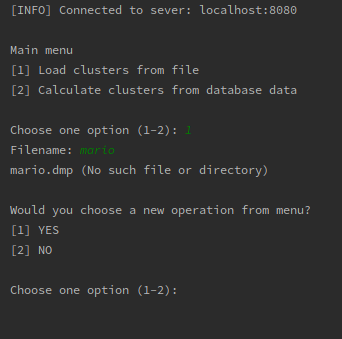
\includegraphics[scale=0.9]{BASE1}
            \caption{L'utente sceglie di caricare i risultati del clustering 
            da file. Prova quindi a caricare un file chiamato "mario" ma il file non
            è presente quindi viene visualizzato un errore. All'utente viene
            chiesto se vuole scegliere una nuova opzione dal menu}   
            \label{fig:1}
        \end{figure}

        \begin{figure}[H]
            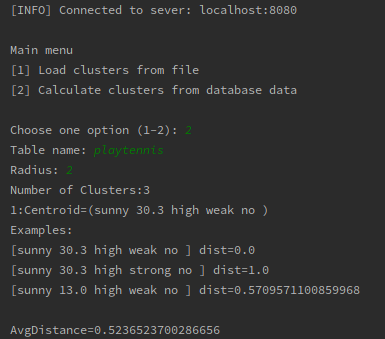
\includegraphics{BASE2}
            \caption{L'utente sceglie di effettuare il clustering su tabella su
            database, inserisce quindi il nome della tabella e il raggio. Nell'
            immagine viene visualizzato solo uno dei tre cluster forniti in output.}   
            \label{fig:2}
        \end{figure}

        \begin{figure}[H]
            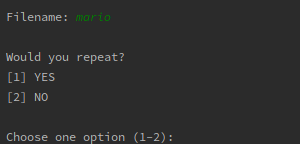
\includegraphics{BASE4}
            \caption{Dopo aver visualizzato i risultati viene chiesto all'
            utente di inserire il nome del file in cui salvare i risultati. L'utente
             puo' decidere di effetuare nuovamente la computazine sulla
            stessa tabella fornendo soltanto il raggio.}   
            \label{fig:3}
        \end{figure}


        \begin{figure}[H]
            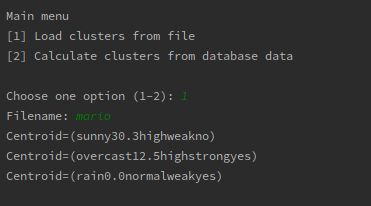
\includegraphics{BASE5}
            \caption{Scegliendo di caricare i cluster da file e inserendo un 
            nome di file corretto vengono visualizzati i dati dei cluster.}   
            \label{fig:4}
        \end{figure} 
        \FloatBarrier
       

    \subsection{Estensione}
    È stato utilizzato il browser Firefox per le prove di utilizzo della 
    applicazione web


    \begin{figure}[H]
        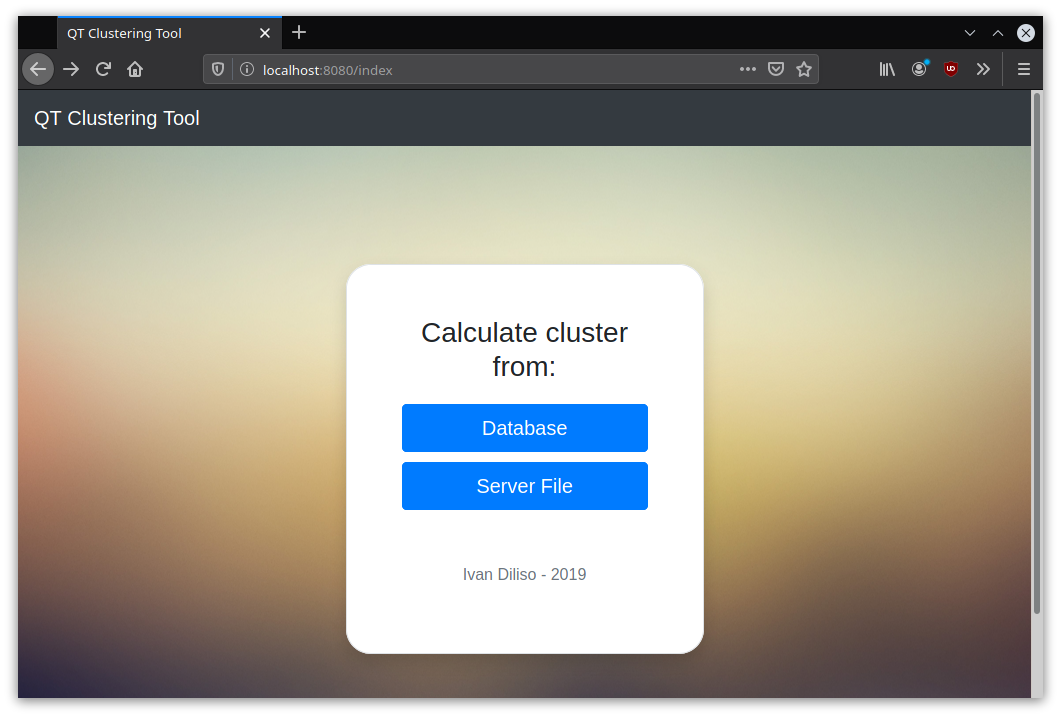
\includegraphics[scale=0.4]{ADDON1}
        \caption{Menu principale, per caricare effettuare il clustering su 
        database cliccare il pulsante "Database", per caricare i risultati del
        clustering da file cliccare il pulsante "Server File"}   
        \label{fig:5}
    \end{figure} 
    \begin{figure}[H]
        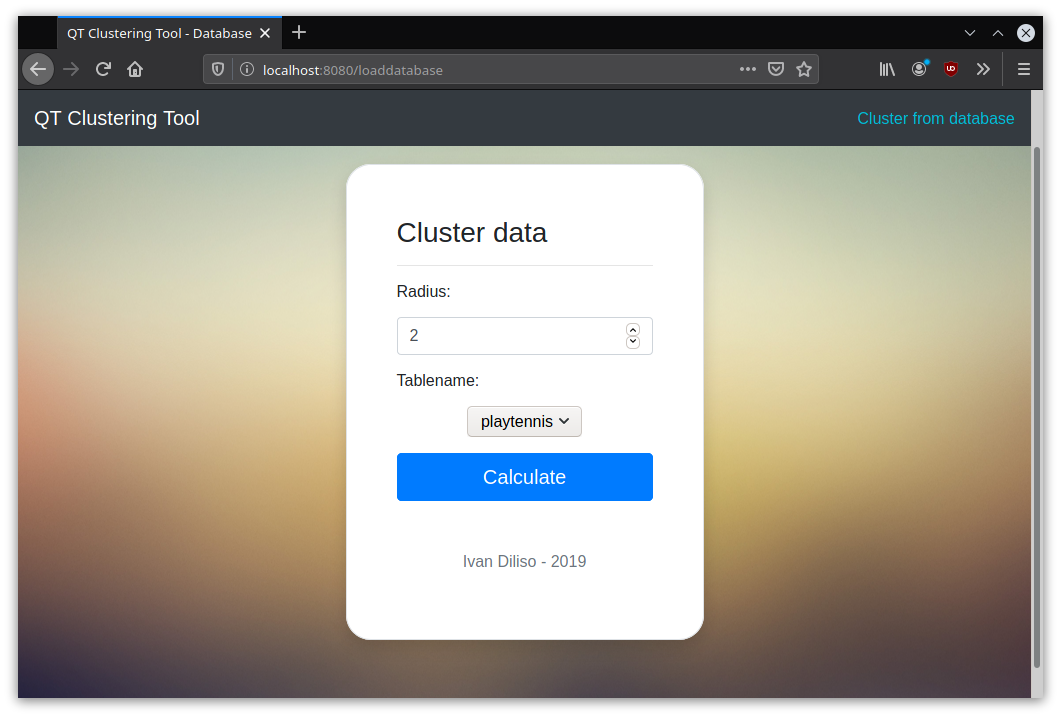
\includegraphics[scale=0.4]{ADDON2}
        \caption{Cliccando il pulsante "Database" si arriva su questa pagina. L'
        utente ha inserito un raggio e ha selezionato dal menu a tendina 
        la tabella da caricare. }   
        \label{fig:6}
    \end{figure} 
    \begin{figure}[H]
        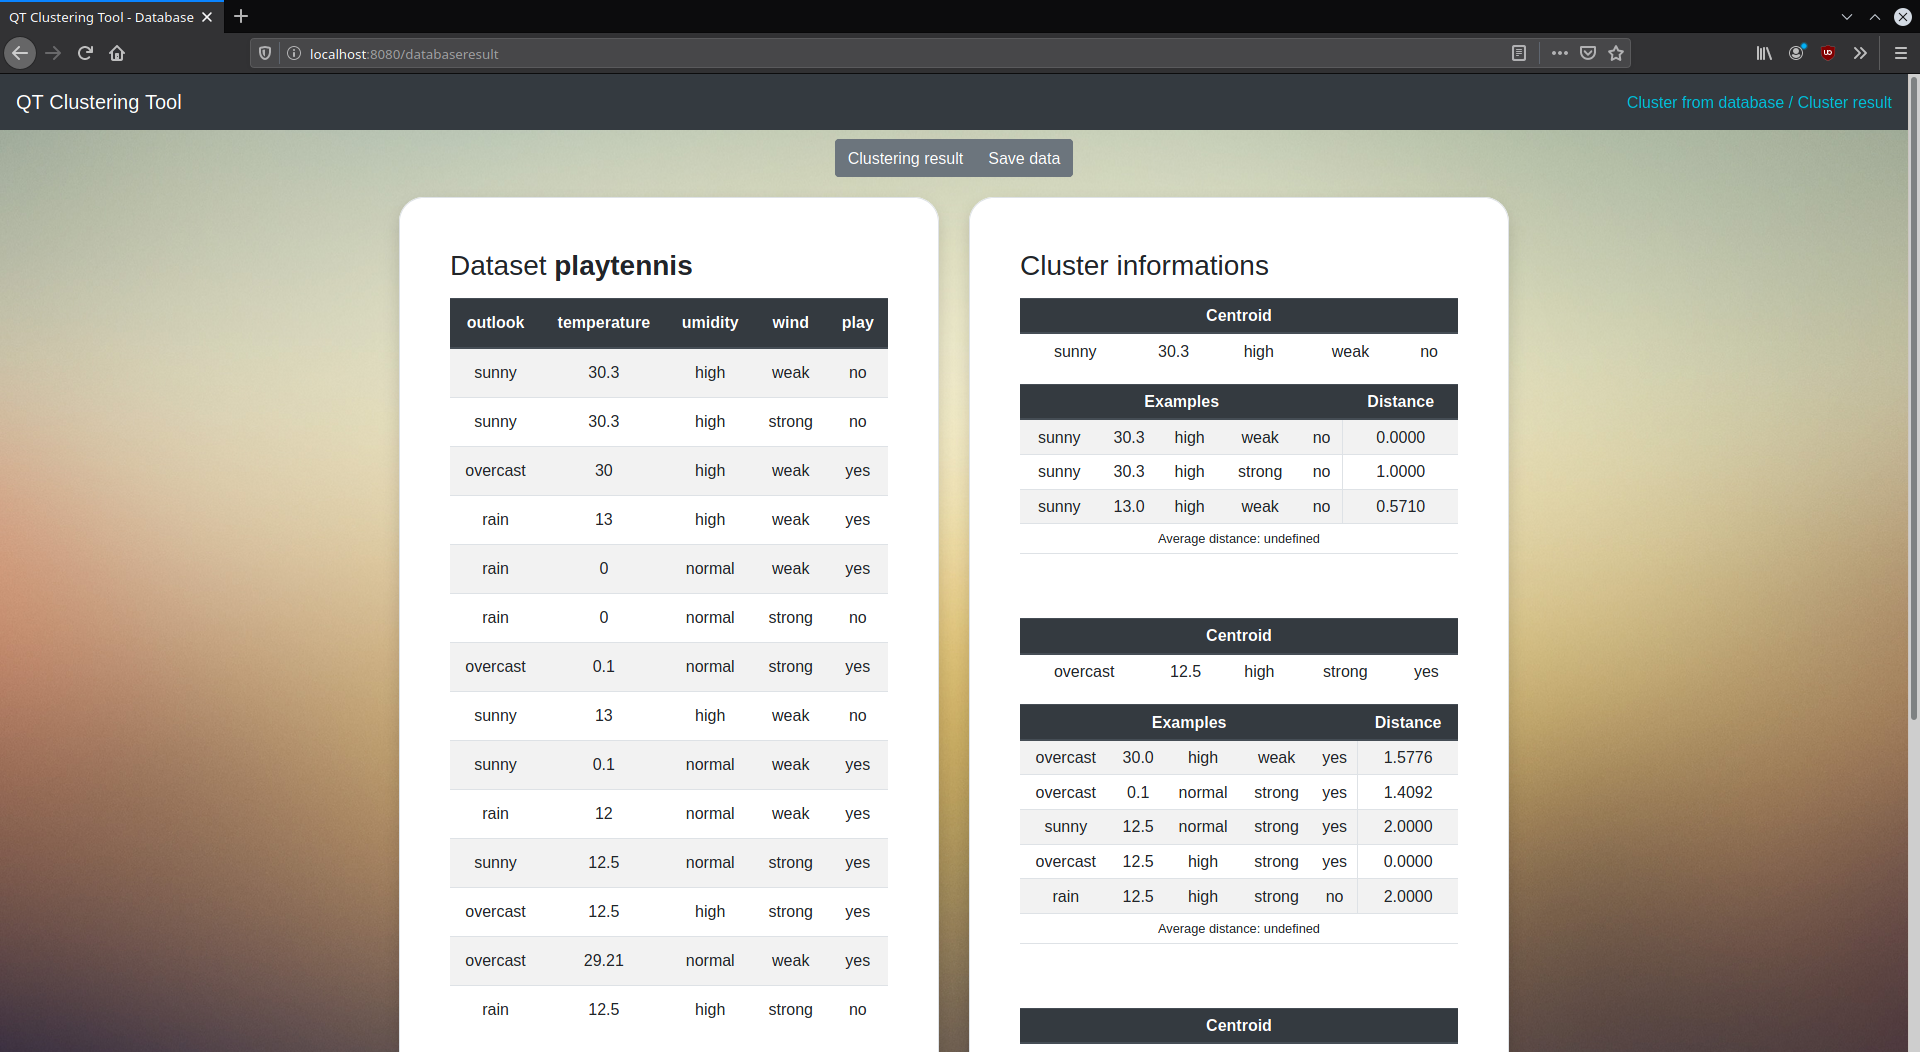
\includegraphics[scale=0.3]{ADDON3}
        \caption{Vengono visualizzati i risultati del clustering. Cliccare su 
        "Save Data" per salvare i risultati su file}   
        \label{fig:7}
    \end{figure} 
    \begin{figure}[H]
        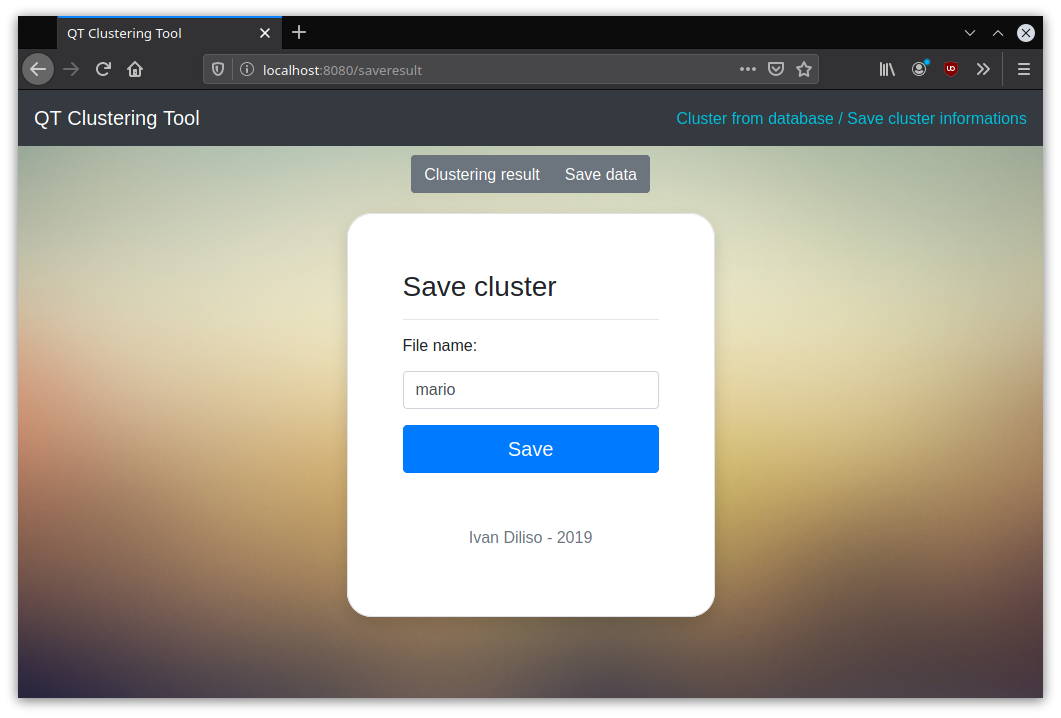
\includegraphics[scale=0.4]{ADDON4}
        \caption{L'utente inserisce il nome del file sul quale salvare i 
        risultati del clustering}   
        \label{fig:8}
    \end{figure} 
    \begin{figure}[H]
        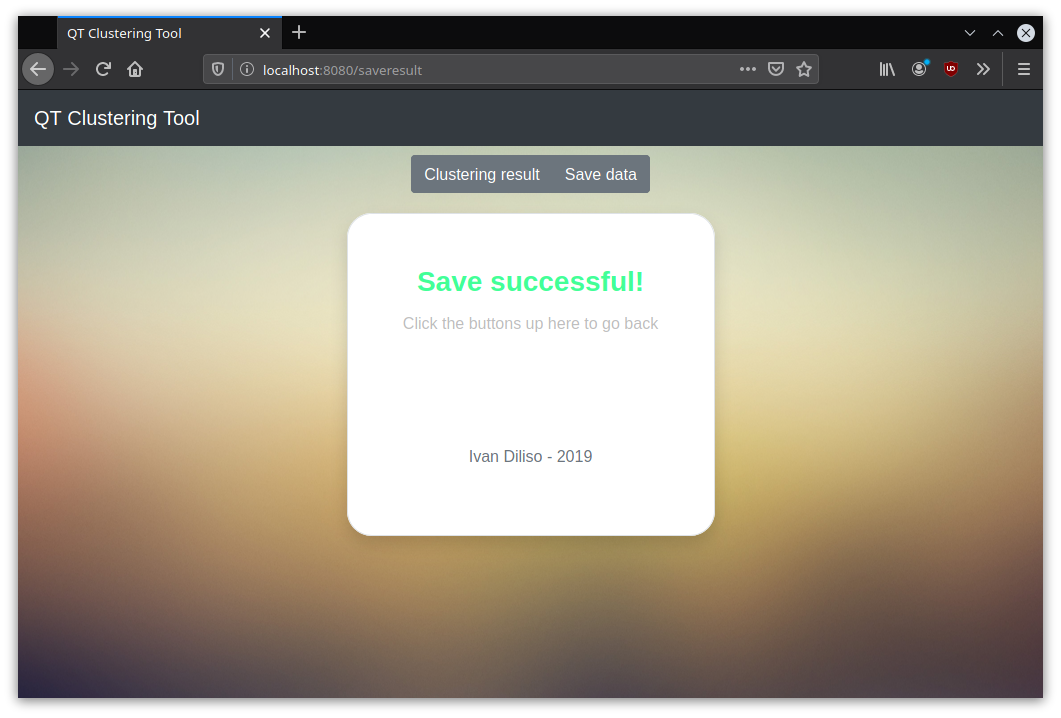
\includegraphics[scale=0.4]{ADDON5}
        \caption{Salvataggio su file avvenuto con successo}   
        \label{fig:9}
    \end{figure} 
    \begin{figure}[H]
        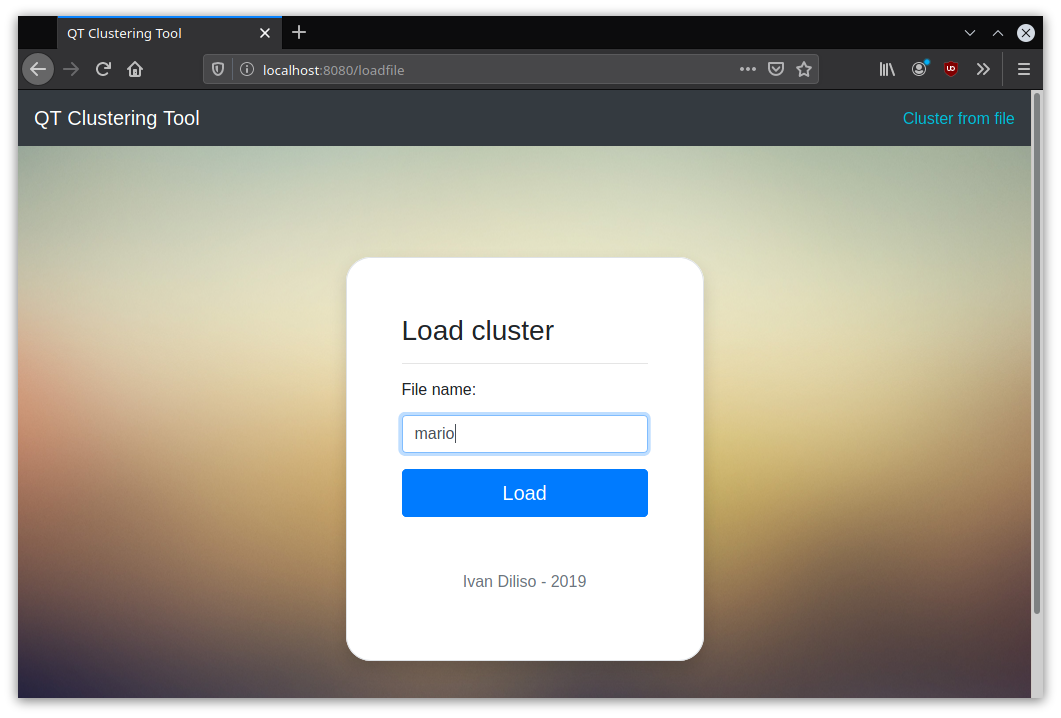
\includegraphics[scale=0.4]{ADDON6}
        \caption{Cliccando su "Server File" nel menu principale si arriva 
        a questa pagina. L'utente inserisce il nome del file dal quale 
        caricare i dati del clustering}   
        \label{fig:10}
    \end{figure} 
    \begin{figure}[H]
        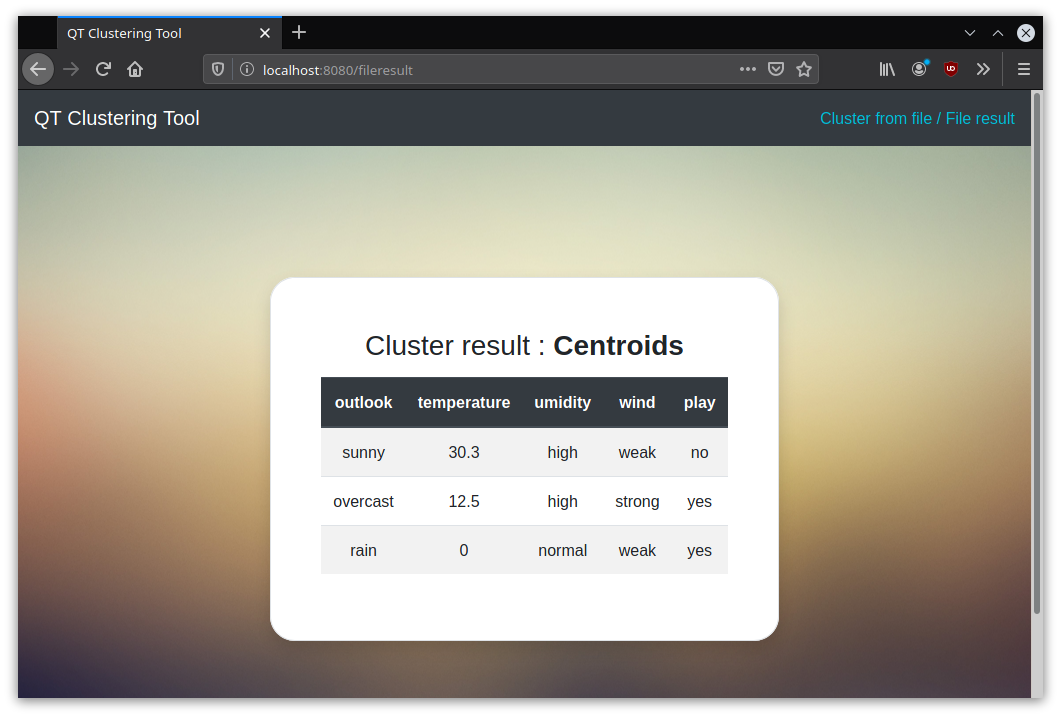
\includegraphics[scale=0.4]{ADDON7}
        \caption{Dati del clustering caricati da file.}   
        \label{fig:11}
    \end{figure} 
    \begin{figure}[H]
        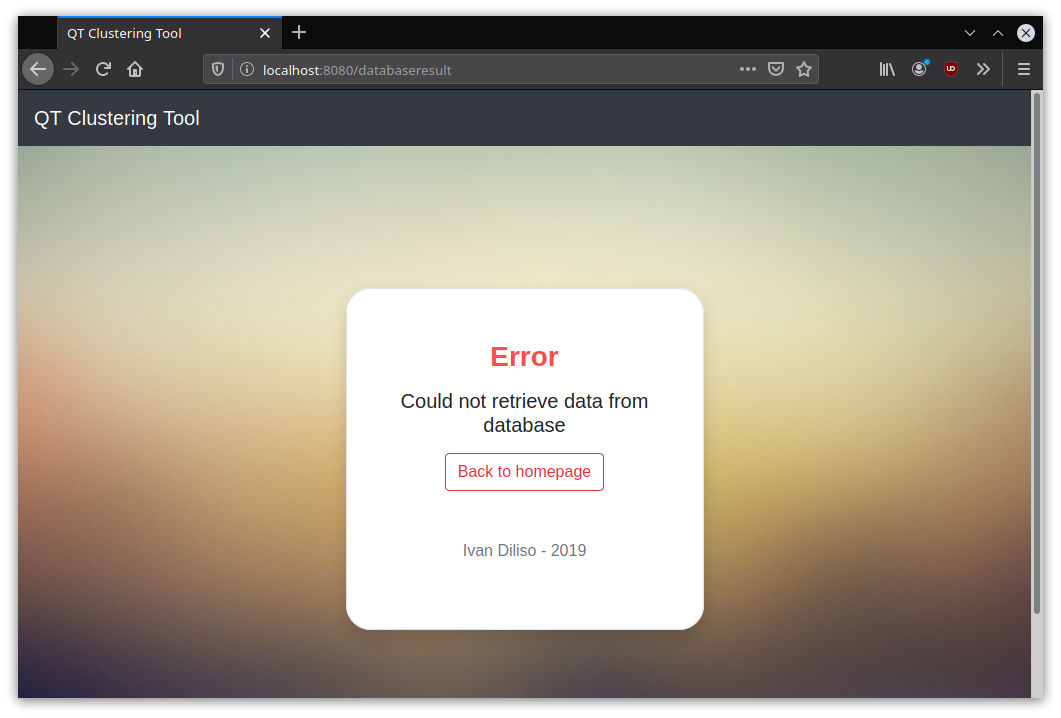
\includegraphics[scale=0.4]{ADDON8}
        \caption{Pagina in cui vengono visualizzati eventuali errori del 
        server. Cliccare sul pulsane "Back to Homepage" per tornare alla 
        Homepage}   
        \label{fig:12}
    \end{figure} 


    \section{Note}
    Nello sviluppo del progetto è stato utilizzato il software 
    \textbf{Git} per il controllo di versione e il software 
    \textbf{Gradle} come sistema di build e gestore delle dipendenze.
    Sono presenti due tabelle per il test dell'applicazione: \verb|playtennis| 
    e \verb|testtable|
        \subsection{Importare il progetto in Eclipse}
        File $>$ Import $>$ Gradle $>$ Existing Gradle Projet $>$ Next $>$
        Selezionare la cartella dei sorgenti QtClient o QtServer o QtWebServer 
        contenute in "Codice sorgente"
        $>$ Next $>$
        Finish
        \subsection{Importare il progetto in IntelliJ  Idea}
        Import Projct $>$
         Selezionare la cartella  QtClient o QtServer o QtWebServer 
         contenute in "Codice sorgente"
         $>$
        Import project from external model $>$ Selezionare Gradle $>$ Finish 

        \subsection{Compilare l'applicazione}
        Utilizzare il task Gradle "build" per compilare l'applicazione, 
        utilizzare il task "run" per avviare l'applicazione. Oppure da linea 
        di comando utilizzare
        il comando \verb|gradlew.bat build| e \verb|gradlw.bat run|. 
        L'output sarà contenuto nella cartella "build".

\end{document}